% Define document class
\documentclass[twocolumn]{aastex631}

\newcommand{\flatiron}{\affiliation{Center for Computational Astrophysics, Flatiron Institute, New York, NY 10010, USA}}
\usepackage{amsmath}
\usepackage{amssymb}
\usepackage{bm}
\usepackage{xcolor}
\definecolor{rb4}{HTML}{27408B}
\newcommand{\kw}[1]{{\color{rb4}[KW: #1 ]}}
\newcommand{\wf}[1]{\textcolor{cyan}{WF: #1}}
% \setlength{\floatsep}{0cm}
% \setlength{\textfloatsep}{0cm}
% \setlength{\belowcaptionskip}{-5pt}
% \setlength{\abovecaptionskip}{-5pt}
% Begin!
\begin{document}
\title{Backpropagating Gravitational wave events}

\pacs{}

\author{Kaze W. K. Wong} 
\email{kwong@flatironinstitute.org}
\flatiron

\author{Katelyn Breivik}
\flatiron

\author{Will Farr}
\flatiron


\date{\today}

\begin{abstract}
Population synthesis simulation is the main workhorse for extracting physical information from a population of gravitational wave (GW) observations.
Unfortunately, current pathways for comparing simulations to observations are not scalable to high dimensionality.
In addition, it is very common to assume a particular distribution for "hyper-parameters" for the entire population (often a fixed value), such as common envelope efficiency.
This limits the flexibility of the model hence potential to discover complex relations between hyper-parameters.
In this work, we introduce a new paradiagm to extract physical information from GW observations.
We propose an inference pipeline to jointly infer the posterior density of both progenitor parameters (e.g. ZAMS masses) and hyper-parameters for each observation in GWTC3.
We showcase the effectiveness of this pipeline with GW150914, as well as its flexibility in studying a population of GW observations. 
\end{abstract}

%\maketitle

\section{Introduction}

As the rate of detection of gravitational-wave (GW) increase with the sensitivity of the GW detector network \kw{cite},
understanding astrophysical processes related to progenitors of GW events through analyzing a population of GW events has become more popular \kw{cite}.
A very common way to study the origin of detected GW events is through population synthesis simulation \kw{cite},
which evolves a population of binaries to form a population of GW events.
Forward modelling of a population of GW events start with sampling a set of initial binary parameters from some distributions related to the progenitor population,
such as the initial mass function or star-formation history,
then evolve each individual members according to the physics of interest until some stopping criteria is met.
This usually mean either a merger event or the binary system stays stable for a Hubble time.
After this, one can collect all the GW emitting binaries in the synthetic population and compare to the observed population.

While forward modelling has been the canonical pathway to simulate binary systems and compare to GW observation,
it is not necessarily the most efficient way to constrain the underlying physical model.
One of the most common skepticism population synthesis studies receives is a simulation set usually only cover a small subdomain of the entire parameter space,
i.e. only vary a number of hyper-parameters (e.g. common envelope efficiency) while holding all others fixed to some "default" values.
Even with recently development on using emulators to speed up the simulation process, training the emulators also require a decent amount of samples in the parameter space of interest.
For example, say we want to emulate a model with 10 parameters, this simplest option for constructing a bank of simulations for training is to lay down a grid.
Along each axis we put the barely minimum of $2$ simulations, this would still require $1024$ simulations.
The fastest kind of population synthesis simulation takes about an hour to complete, where longer simulations could take days.
This means even training an emulator is impossible in a high dimensional space.
To make the problem even worse, there is no gaurantee the entire population should share the same hyper-parameters (i.e. a delta distribution at a fixed value.),
which means there could be a large (possibly infinite) family of hyper-parameters distribution one need to test to compare the simulations to the observed data.

However, this issue is not a fundamental issue, but an apparent obstacle because we are approach the problem from an infinitely inefficient angle.
Since each binary system could in principle come from a different environment, hence they can have different progenitor parameters as well as hyper-parameters.
What one should do is to ask what is the posterior density in the progenitor and hyper-parameter joint space for each individual binary system,
then perform population analysis in that space.
In this paper, we propose a method to "backward" model each GW event to its progenitor state.
The method is a two stages process:
first we solve a root finding problem to obtain guesses that are likely to produce the desire system properties in the joint space,
then we sample the posterior in the joint space with Markov chain Monte Carlo (MCMC) algorithm that is initialized using the root found in the previous stage.
This paper is structured as follows: We detail our method in Sec. ~\ref{sec:method}.
In Sec. ~\ref{sec:result}, we show the results of applying our method to a number of real events.
We discuss the implications of this work and future direction in Sec. ~\ref{sec:discussion}.

\section{Method}
\label{sec:method}

We define the parameters that describe the progenitor's properties such as ZAMS
masses and eccentricity as progenitor parameters $\bm{\theta'}$, the parameters
that control different physical prescriptions such as wind strength and common
envelope efficiency as hyper-parameters $\bm{\lambda}$, and random variables
that affect certain stochastic process such as whether natal kick unbinds a
binary as $\bm{X}$. To avoid clutter in the following derivation, we denote all
the parameters related to mapping a particular progenitor system into a GW event
collectively as evolutionary parameters $\bm{\Theta}$, which includes
$\bm{\theta'}$, $\bm{\lambda}$, and $\bm{X}$.

Once all the parameters including a particular draw of all the random variables
represented by $\bm{X}$ are known, the population synthesis code is a
deterministic function that transforms the properties of the progenitors into
the GW parameters $\bm{\theta}$:
\begin{equation}
    \bm{\theta} = \bm{f}\left( \bm{\Theta} \right).
\end{equation}
The mapping $\bm{f}$ from $\bm{\Theta}$ to $\bm{\theta}$ can be many-to-one.  
In order to draw inferences about $\bm{\Theta}$ from gravitational wave data, we
need to be able to evaluate the likelihood of that data at fixed progenitor
parameters, namely
\begin{equation}
    p\left( d \mid \bm{\Theta} \right) = p\left( d \mid \bm{\theta} = \bm{f}\left( \bm{\Theta} \right) \right).
\end{equation}
The equality holds because the likelihood depends only on the gravitational waveform generated by
parameters $\bm{\theta}$ to which the progenitor parameters map onto.  In principle
this likelihood could be computed at arbitrary values of $\bm{\Theta}$ using the
same machinery that is used to estimate source parameters in gravitational wave
catalogs \citep{Veitch2015,Ashton2019,Romero-Shaw2020,GWTC-3} to develop samples
of progenitor parameters, hyper-parameters, and random variables in
$\bm{\Theta}$ from a posterior density.

Since the gravitational wave likelihood function
ultimately depends only on the GW parameters $\theta$, and GWTC3 already has samples over these parameters from a posterior density 
\begin{equation}
    p\left( \bm{\theta} \mid d \right) \propto p\left( d \mid \bm{\theta} \right) \pi_\mathrm{GW} \left( \bm{\theta} \right),
\end{equation}
where $\pi_\mathrm{GW}$ is the prior density used for sampling,
we can save the computation cost in evaluating the GW likelihood by rewriting the posterior density of $\Theta$ in terms of the posterior density of $\theta$, namely

\begin{align}
    p(\Theta | d) = \frac{p(\theta(\Theta)| d) \pi(\Theta)}{\pi_\mathrm{GW}(\theta(\Theta))},
\end{align}
which we applies a kernel density estimator to the posterior samples released in GWTC3 to estimate $p(\theta(\Theta)|d)$.

Including hyper-parameters and random variables in the sampling drastically increase the dimensionality of the problem,
which makes the sampling process more computationally expensive and harder to converge.
To speed up the convergence, we first solve a root-finding problem to find points that are close to the bulk of the posterior density,
then we use those points to initialize a set of chains in the MCMC process.


The root-finding procedure is described as followed:
For each posterior sample point in the GW observables space,
we can find the corresponding evolutionary parameters by solving an optimization problem that minimize the mean square difference between the GW event parameters and evolutionary parameters, i.e. 

\begin{align}
\mathcal{L}(\bm{\Theta},\bm{\theta}) = ||f(\bm{\Theta})-\bm{\theta}||^2
\label{eq:loss}
\end{align}

In principle, we should only accept solutions that exactly reproduce the LVK posterior samples in the observable space.
However, it is not feasible to achieve such condition in practice, therefore we relax the condition in eq.\ref{eq:loss} to a small acceptance threshold, in our case we picked $10^{-2}$ to be our threshold.
To make sure we find a reasonably complete set of progenitor parameters that corresponds to the posterior sample point, we use 1000 different initial guesses in solving the optimization problem.
As long as the solution fulfill the acceptance criteria, the root is as valid as all other roots that fulfill the same acceptance criteria, regardless to its initial guess.
In other word, we have the freedom to choose the set of initial guesses however we think it might benefit the optimization.
Most of the points in the evolutionary parameter space do not produce mergers, and for systems that do not merge, we set the binary masses to be 0.
This means the gradient for systems that do not merge is 0, and the root finder would likely to get stuck in such state during the first step.\footnote{On a plateau of constant loss, the root finder performs no better than a random guess. In a high dimensional space, this means the root finder will need a long time to get close to a solution.}
Therefore, it is beneficial to put initial guesses in region of the evolutionary parameter space that does produce merger.
To construct a list of initial guesses, we evolve a set of points that we uniformly sampled from the evolutionary parameter space, then keep the points that merge within a Hubble time.

Ideally we would like to have explicit control over all evolutionary parameters.
In particular, having explicit control over random variables allows us to marginalize over their contribution, so we can focus on progenitor parameters and hyper-parameters.
However, in practice most of the population synthesis simulation code (including \texttt{COSMIC} which we use in this study.) define their random variables implicitly,
i.e. the random variables are drawn within the program, instead of being arguments of the program.
This means the function we use to evolve the binary is not a deterministic function but a stochastic function instead. 
Hence, even if the root-finding algorithm performs perfectly,
forward modelling this set of roots does not guarantee to reproduce the set of posterior samples due to randomness of the evolution function.
To assure the recovered progenitor and hyper-parameters robustly corresponds to the posterior in the GW observables space,
we forward model ("Reproject") the recovered evolutionary parameters to the observables space to check whether the reprojected posterior agrees with the posterior given by the LVK collaboration.
We use KL divergence to measure the agreement between the two posterior distributions, which is given by
\begin{align}
D_{KL}(P||Q) = \int P(\bm{x}) \log(P(\bm{x})/Q(\bm{x})) dx.
\label{eq:KLdivergence}
\end{align}

A small KL divergence means the reprojected \texttt{COSMIC} posterior is similar to the original posterior in the observable space, hence it is a viable channel for that specific event, otherwise it either means \texttt{COSMIC} can only explain part of the posterior or cannot explain the event at all.
This is completely expected since \texttt{COSMIC} comes with its own assumptions and is expected to fail in reproducing a subset of the event in GWTC3, such as event with at least one component beyond the pair instability supernova massgap.
On the other hand, the reprojection could subject to stochasticity in the evolution function we use.
Instead of reprojecting the posterior only once, we reproject the posterior multiple times with different random seeds and check whether the KL divergence varies significantly.
A varying KL divergence means this particular event is subjected to randomness in the evolution function, hence one should take extra caution in interpreting the result.


\section{Result}
\label{sec:result}

\begin{table*}[hbt!]
    \begin{center}
    \begin{tabular}{ l l l }
    \hline
    \hline
    Parameters &  Description & Optimization range\\
    \hline
    \hline
    Observables &\ &\  \\
    \hline
    \hline
    $M_{\rm GW,1}$ & Primary mass of the GW event & NA \\
    $M_{\rm GW,2}$ & Secondary mass of the GW event  & NA\\
    \hline
    \hline
    Progenitor parameters &\ &\  \\
    \hline
    \hline
    $M_{\rm ZAMS,1}$ & Primary mass at ZAMS & $[10,150]\ M_{\odot}$\\
    $M_{\rm ZAMS,2}$ & Secondary mass at ZAMS & $[10,150]\ M_{\odot}$\\
    $t_{\rm orb}$ & Orbital period at ZAMS & $[5,5000]$ days\\
    $e$ & Eccentricity at ZAMS & $[0,1]$\\
    $Z$ & Metallicity at ZAMS & $[10^{-4},2\times10^{-2}]$\\
    $z$ & Redshift at ZAMS & NA\\
    \hline
    \hline
    Hyper-parameters &\ &\ \\
    \hline
    \hline
    
    $\alpha$ & Common envelope efficiency & $[0.1,10]$\\
    $f_{\rm acc}$ & Fraction of accretion during stable mass transfer & $[0,1]$\\
    $q_{\rm crit,3}$ & \kw{Katie fill in} & $[0.1,10]$\\
    $\sigma$ & \kw{Katie fill in}& $[10,300]\ {\rm km/h}$\\


    \hline
    \hline
    \end{tabular}
    \caption{A list of parameters we used in this study.}
    \label{tab:parameters}
    \end{center}
\end{table*}
    
We apply the method described in section \ref{sec:method} to the first GW events GW150914.
The parameters involved in the analysis and the range we allow for finding the root are tabulated in table \ref{tab:parameters}.
\kw{@Katie state why not spin here.}
Therefore, we solve the rootfinding problem with only the two component masses in the observable space.
For progenitor parameters, we characterize each guess with five parameters: the two component masses $M_{\rm ZAMS,1}$ and $M_{\rm ZAMS,2}$, the orbital period $t_{\rm orb}$, the eccentricity $e$, the metallicity $Z$ at ZAMS.
Note that the progenitor formation redshift is not obtained through the root-finding process.
This is because the formation redshift does not affect the evolution of the binary, so we do not need to include in the optimization.
Instead, we compute the time it takes for the binary to evolve from formation to the merger, then we add this time back to the lookback time when this event is observed.
Using the total lookback time, we can compute the redshift of the binary at formation.
We adopt the cosmological model in \kw{cite Planck 18} to compute the redshift of the binary at formation.
For hyper-parameters, we choose parameters that affect binary evolution in \texttt{COSMIC} mostly significantly, including the common envelope efficiency $\alpha$, the fraction of accretion during stable mass transfer $f_{\rm acc}$, the critical mass fraction $q_{\rm crit,3}$, and the accretion rate $\sigma$.
We show a portion of the joint posterior of the progenitor parameters and hyper-parameters of GW150914 in figure \ref{fig:GW150914_posterior}.

\kw{Recover ratio of the posterior sample goes here.}

The full posterior is available in appendix \kw{Or we should put a link to the dataset?}

\begin{figure*}[h]
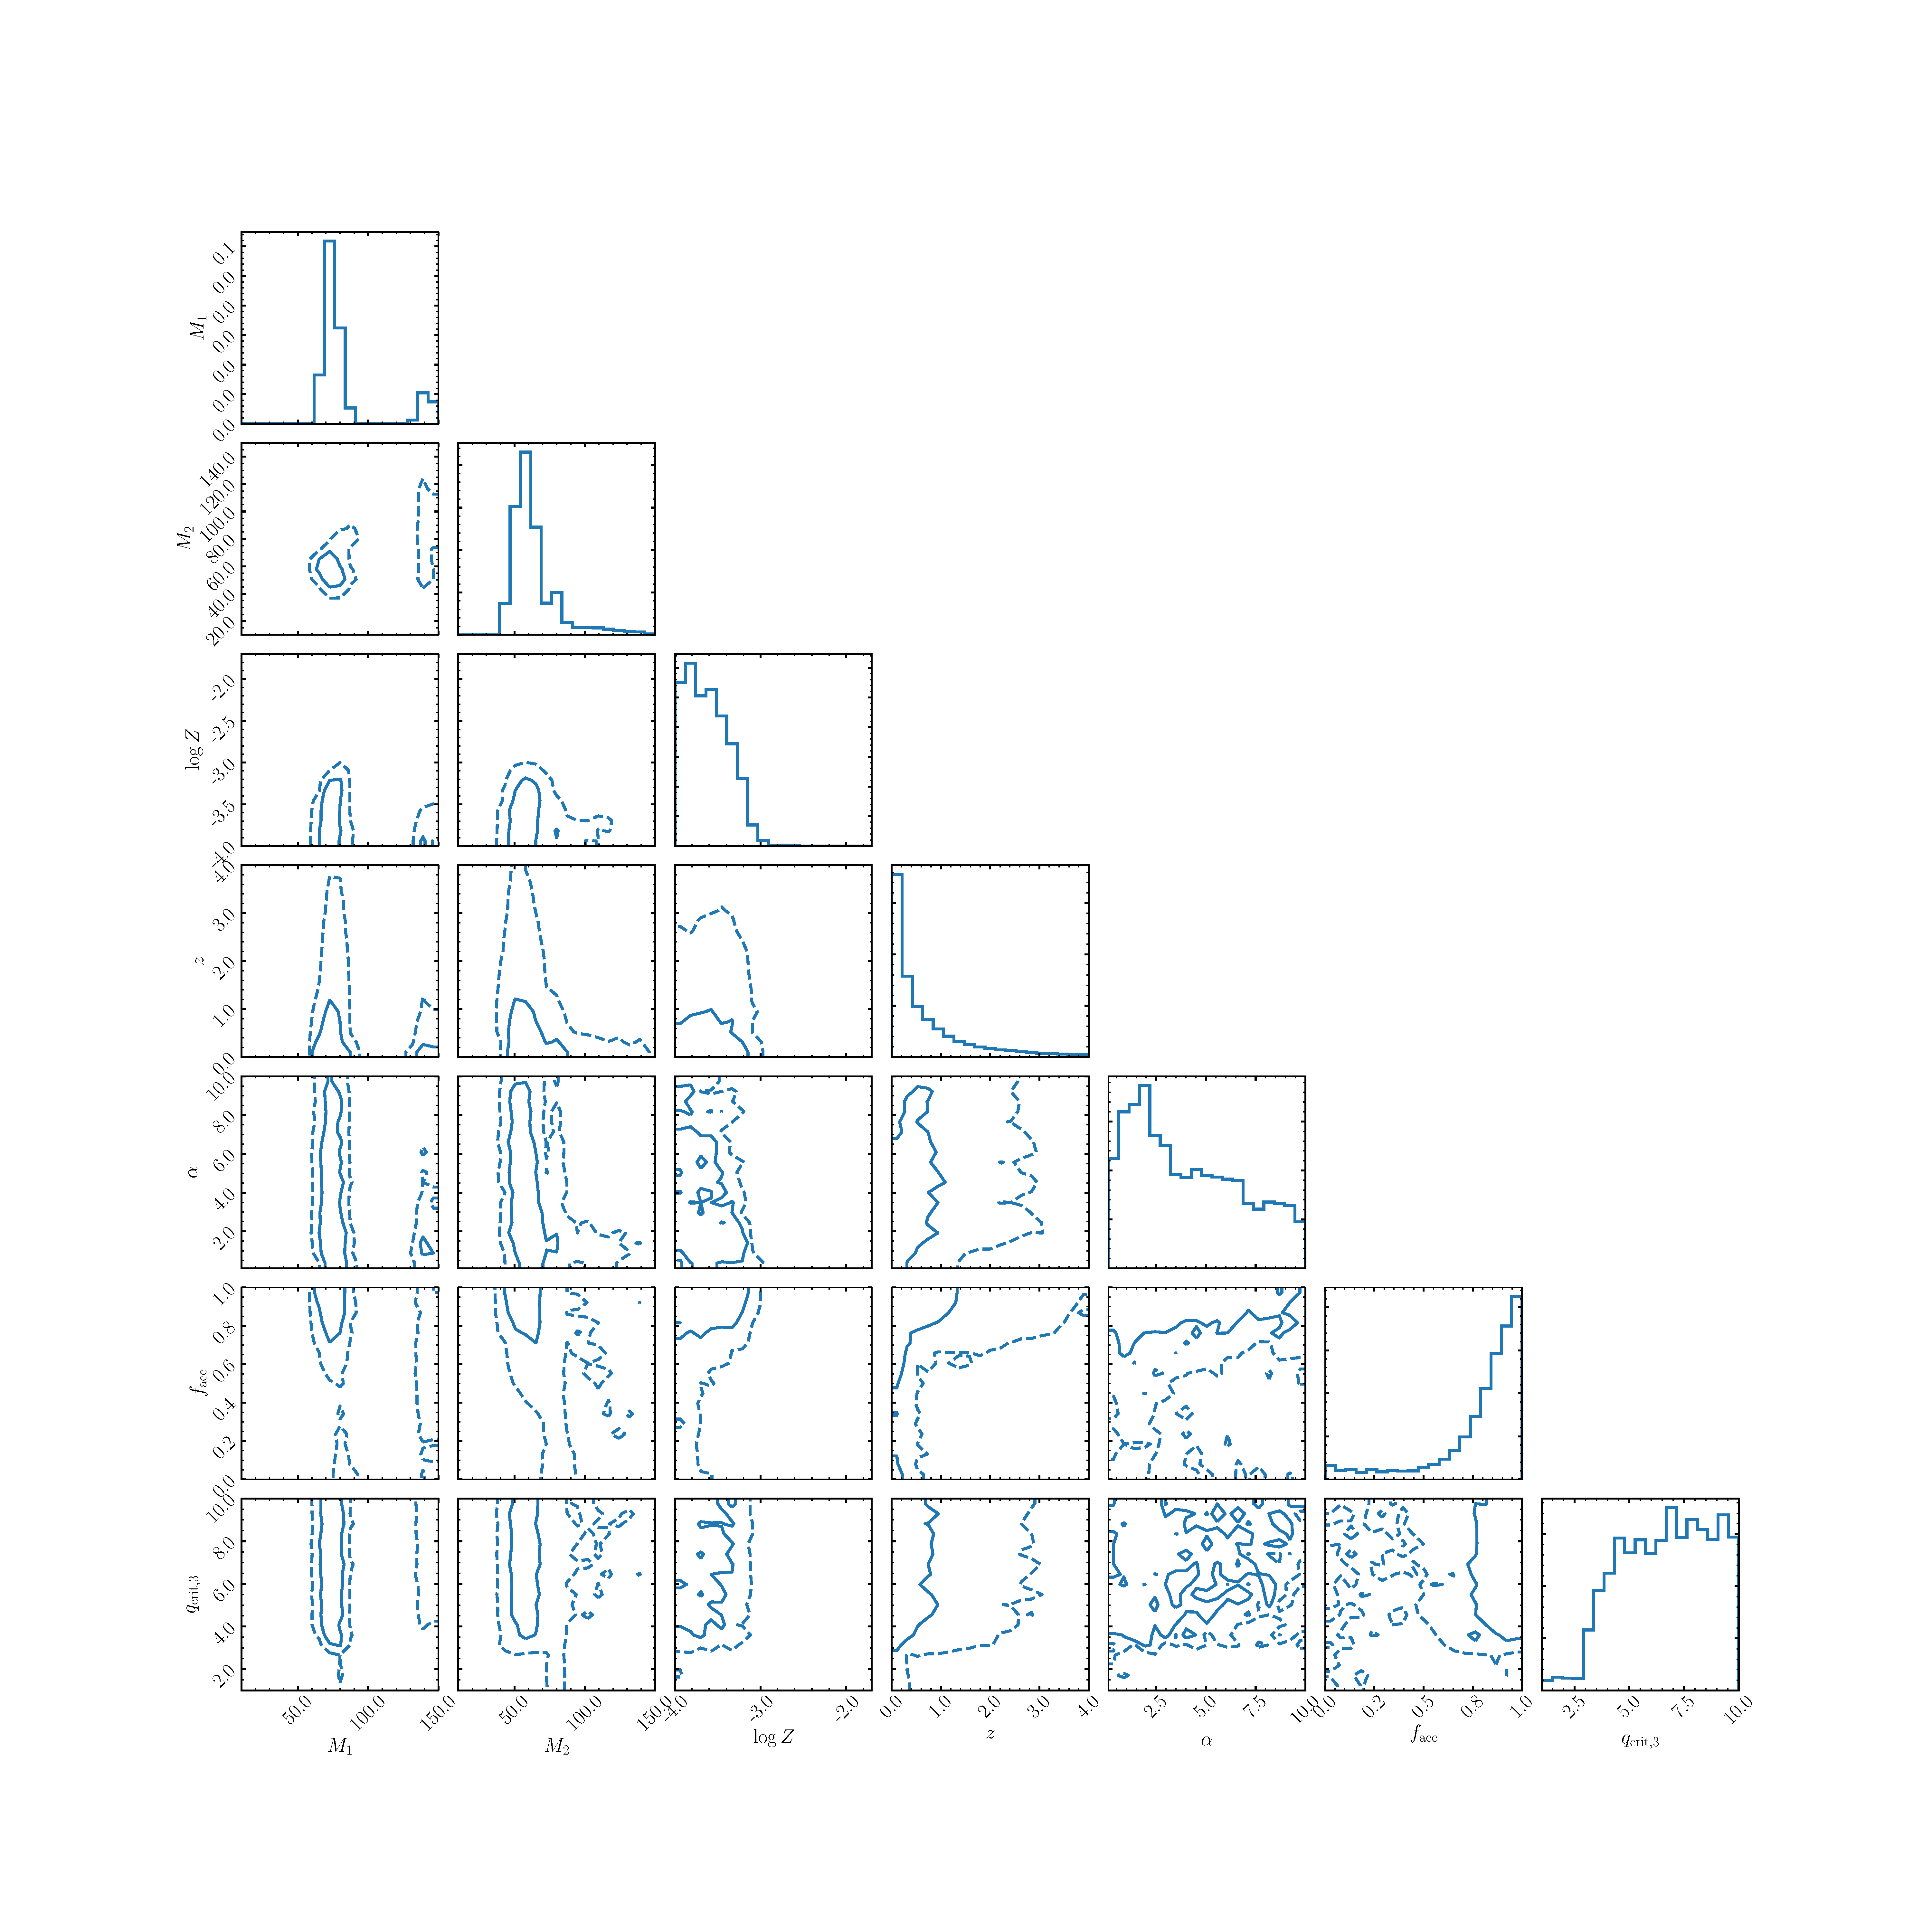
\includegraphics[width=\textwidth]{static/GW150914_corner_zoomed.pdf}
\caption{The posterior for GW150914 in both the progenitor parameter space and hyper-parameter space.
$M_1$ and $M_2$ are the progenitors' masses. $\log{Z}$ is log metallicity at ZAMS.
$z$ is the redshift at ZAMS. 
$\alpha$ is the common envelope efficiency.
$f_{\rm acc}$ is the fraction of mass accreted during stable mass transfer.
$q_{\rm crit 3}$ are the critical mass during \kw{Katie fill in},
Note that the redshift is not fitted during the root finding process.
Once we have find the evolutionary parameters, we add the time it would take the progenitor to merge to the lookback time of the observed posterior sample,
then from the total lookback time we can compute the redshift at ZAMS.
}
\label{fig:GW150914_posterior}
\end{figure*}

To check the validity of the recovered posterior, it is essential to check whether it is consistent with the original posterior in the observable space.
We reproject the recovered posterior to the observable space, and compare the KL divergence between the original posterior and the reprojected posterior.
For GW150914, the KL divergence between the reprojected posterior and the original posterior is \kw{fill later} on average.
The KL divergence stays stable for reprojecting with different random seeds.

\begin{figure}
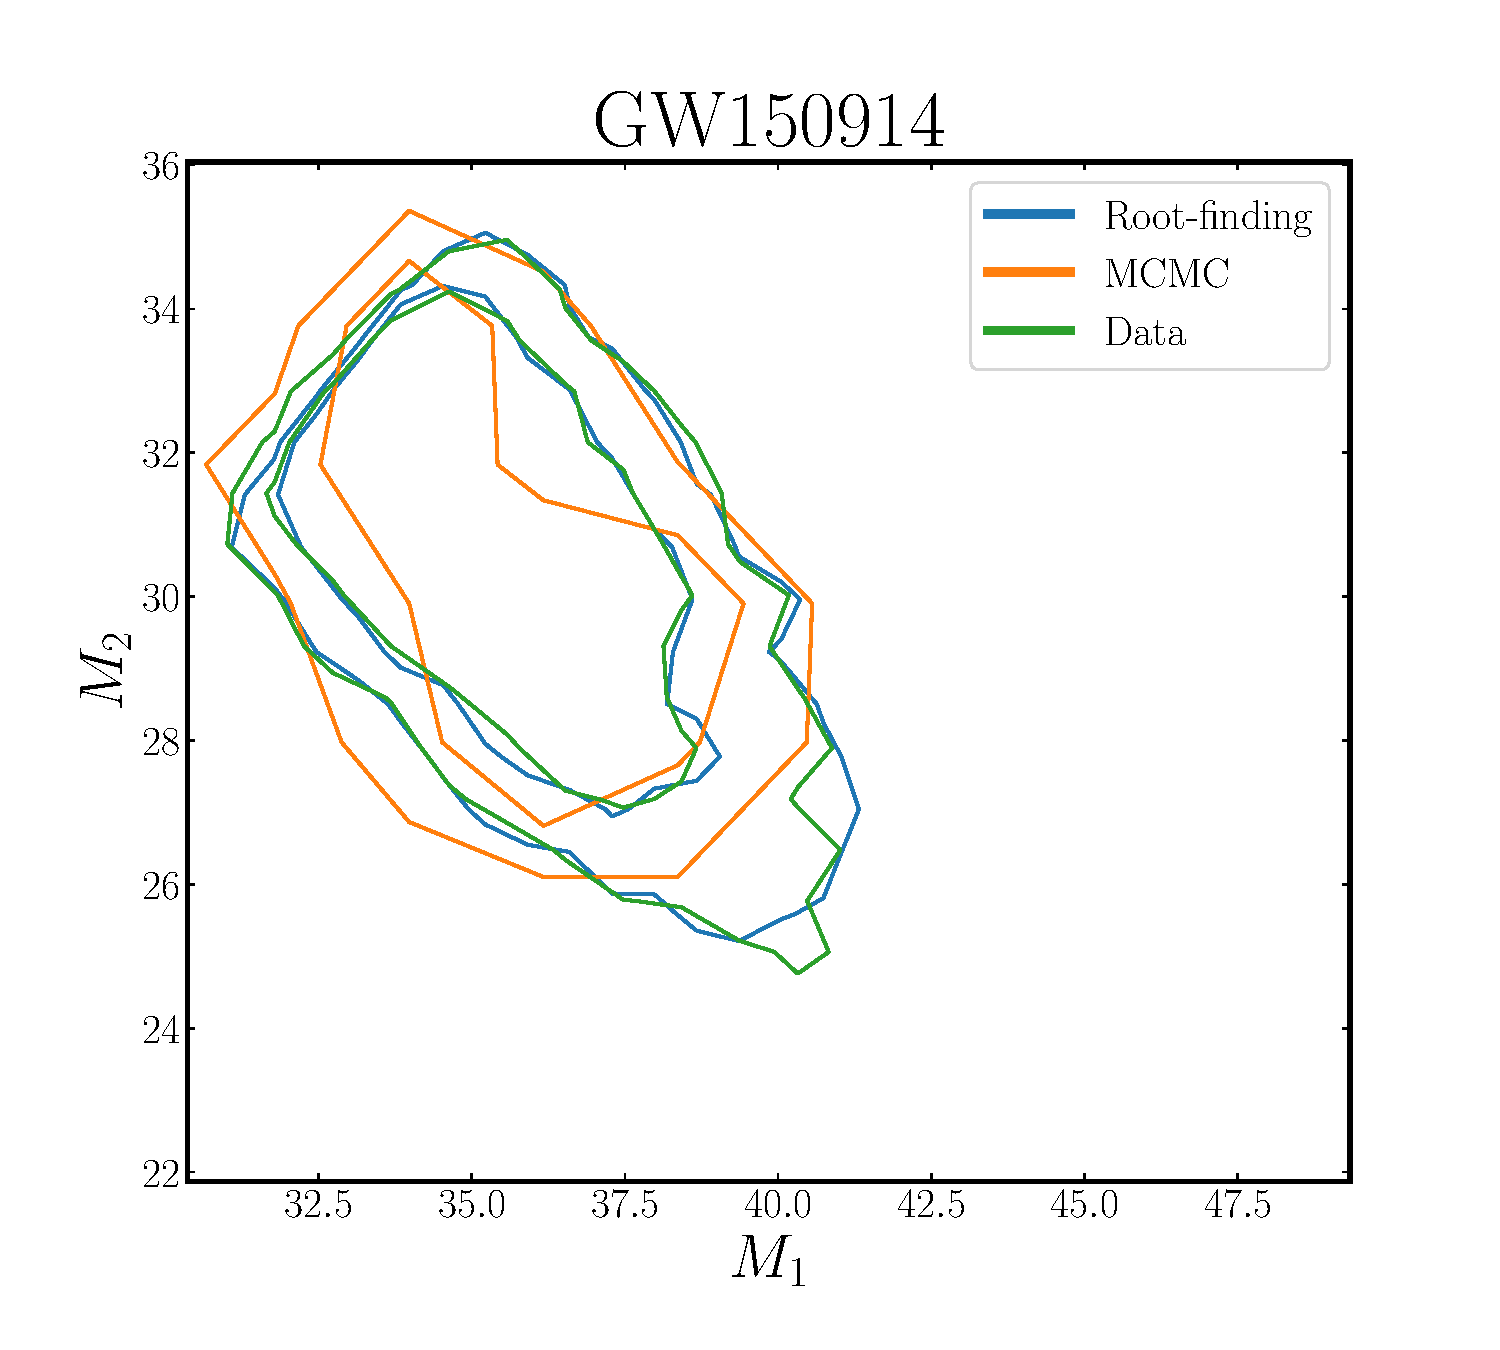
\includegraphics[width=0.49\textwidth]{static/GW150914_reprojection.pdf}
\caption{Reprojecting the posterior in evolutionary parameter space of GW150914 to observable space.
The blue contour is the posterior reprojected using the samples in the evolutionary parameter space.
The orange contour is the posterior samples from LVK that have corresponding samples in the evolutionary parameter space.
The green contour is the posterior plotted using all of LVK posterior samples.
}
\label{fig:GW150914_reprojection}
\end{figure}
We can see the reprojected posterior agrees very well with the original posterior in fig.\ref{fig:GW150914_reprojection}.


% \begin{figure}
% 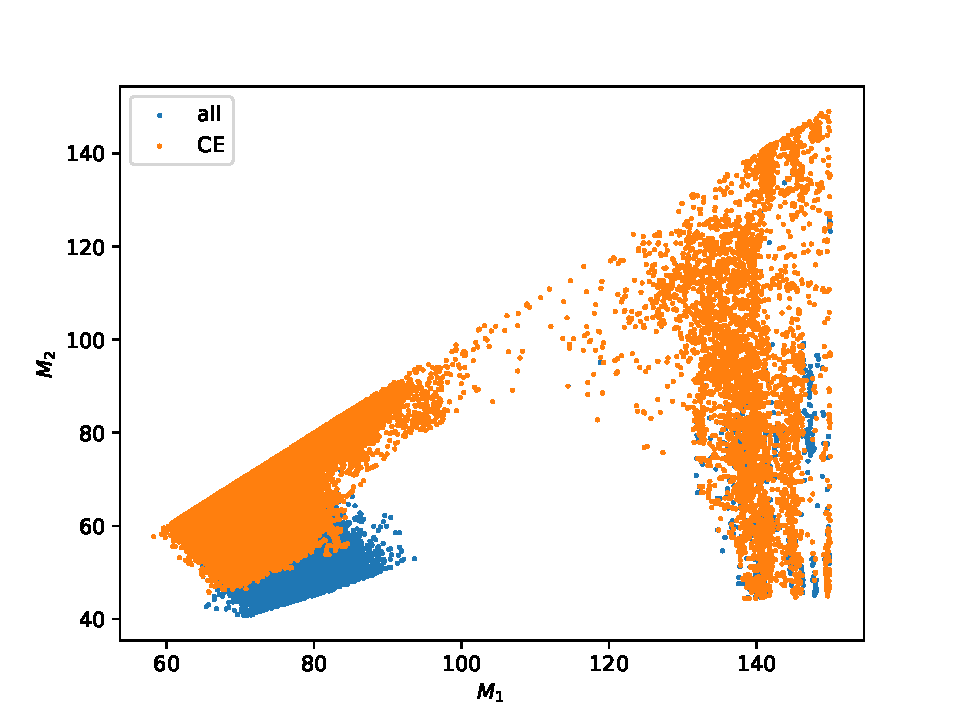
\includegraphics[width=0.49\textwidth]{static/GW150914_CE_SMT.pdf}
% \caption{}
% \label{fig:GW150914_CE_SMT}
% \end{figure}
% \kw{Add figure of stable mass transfer vs common envelope}

\begin{figure}
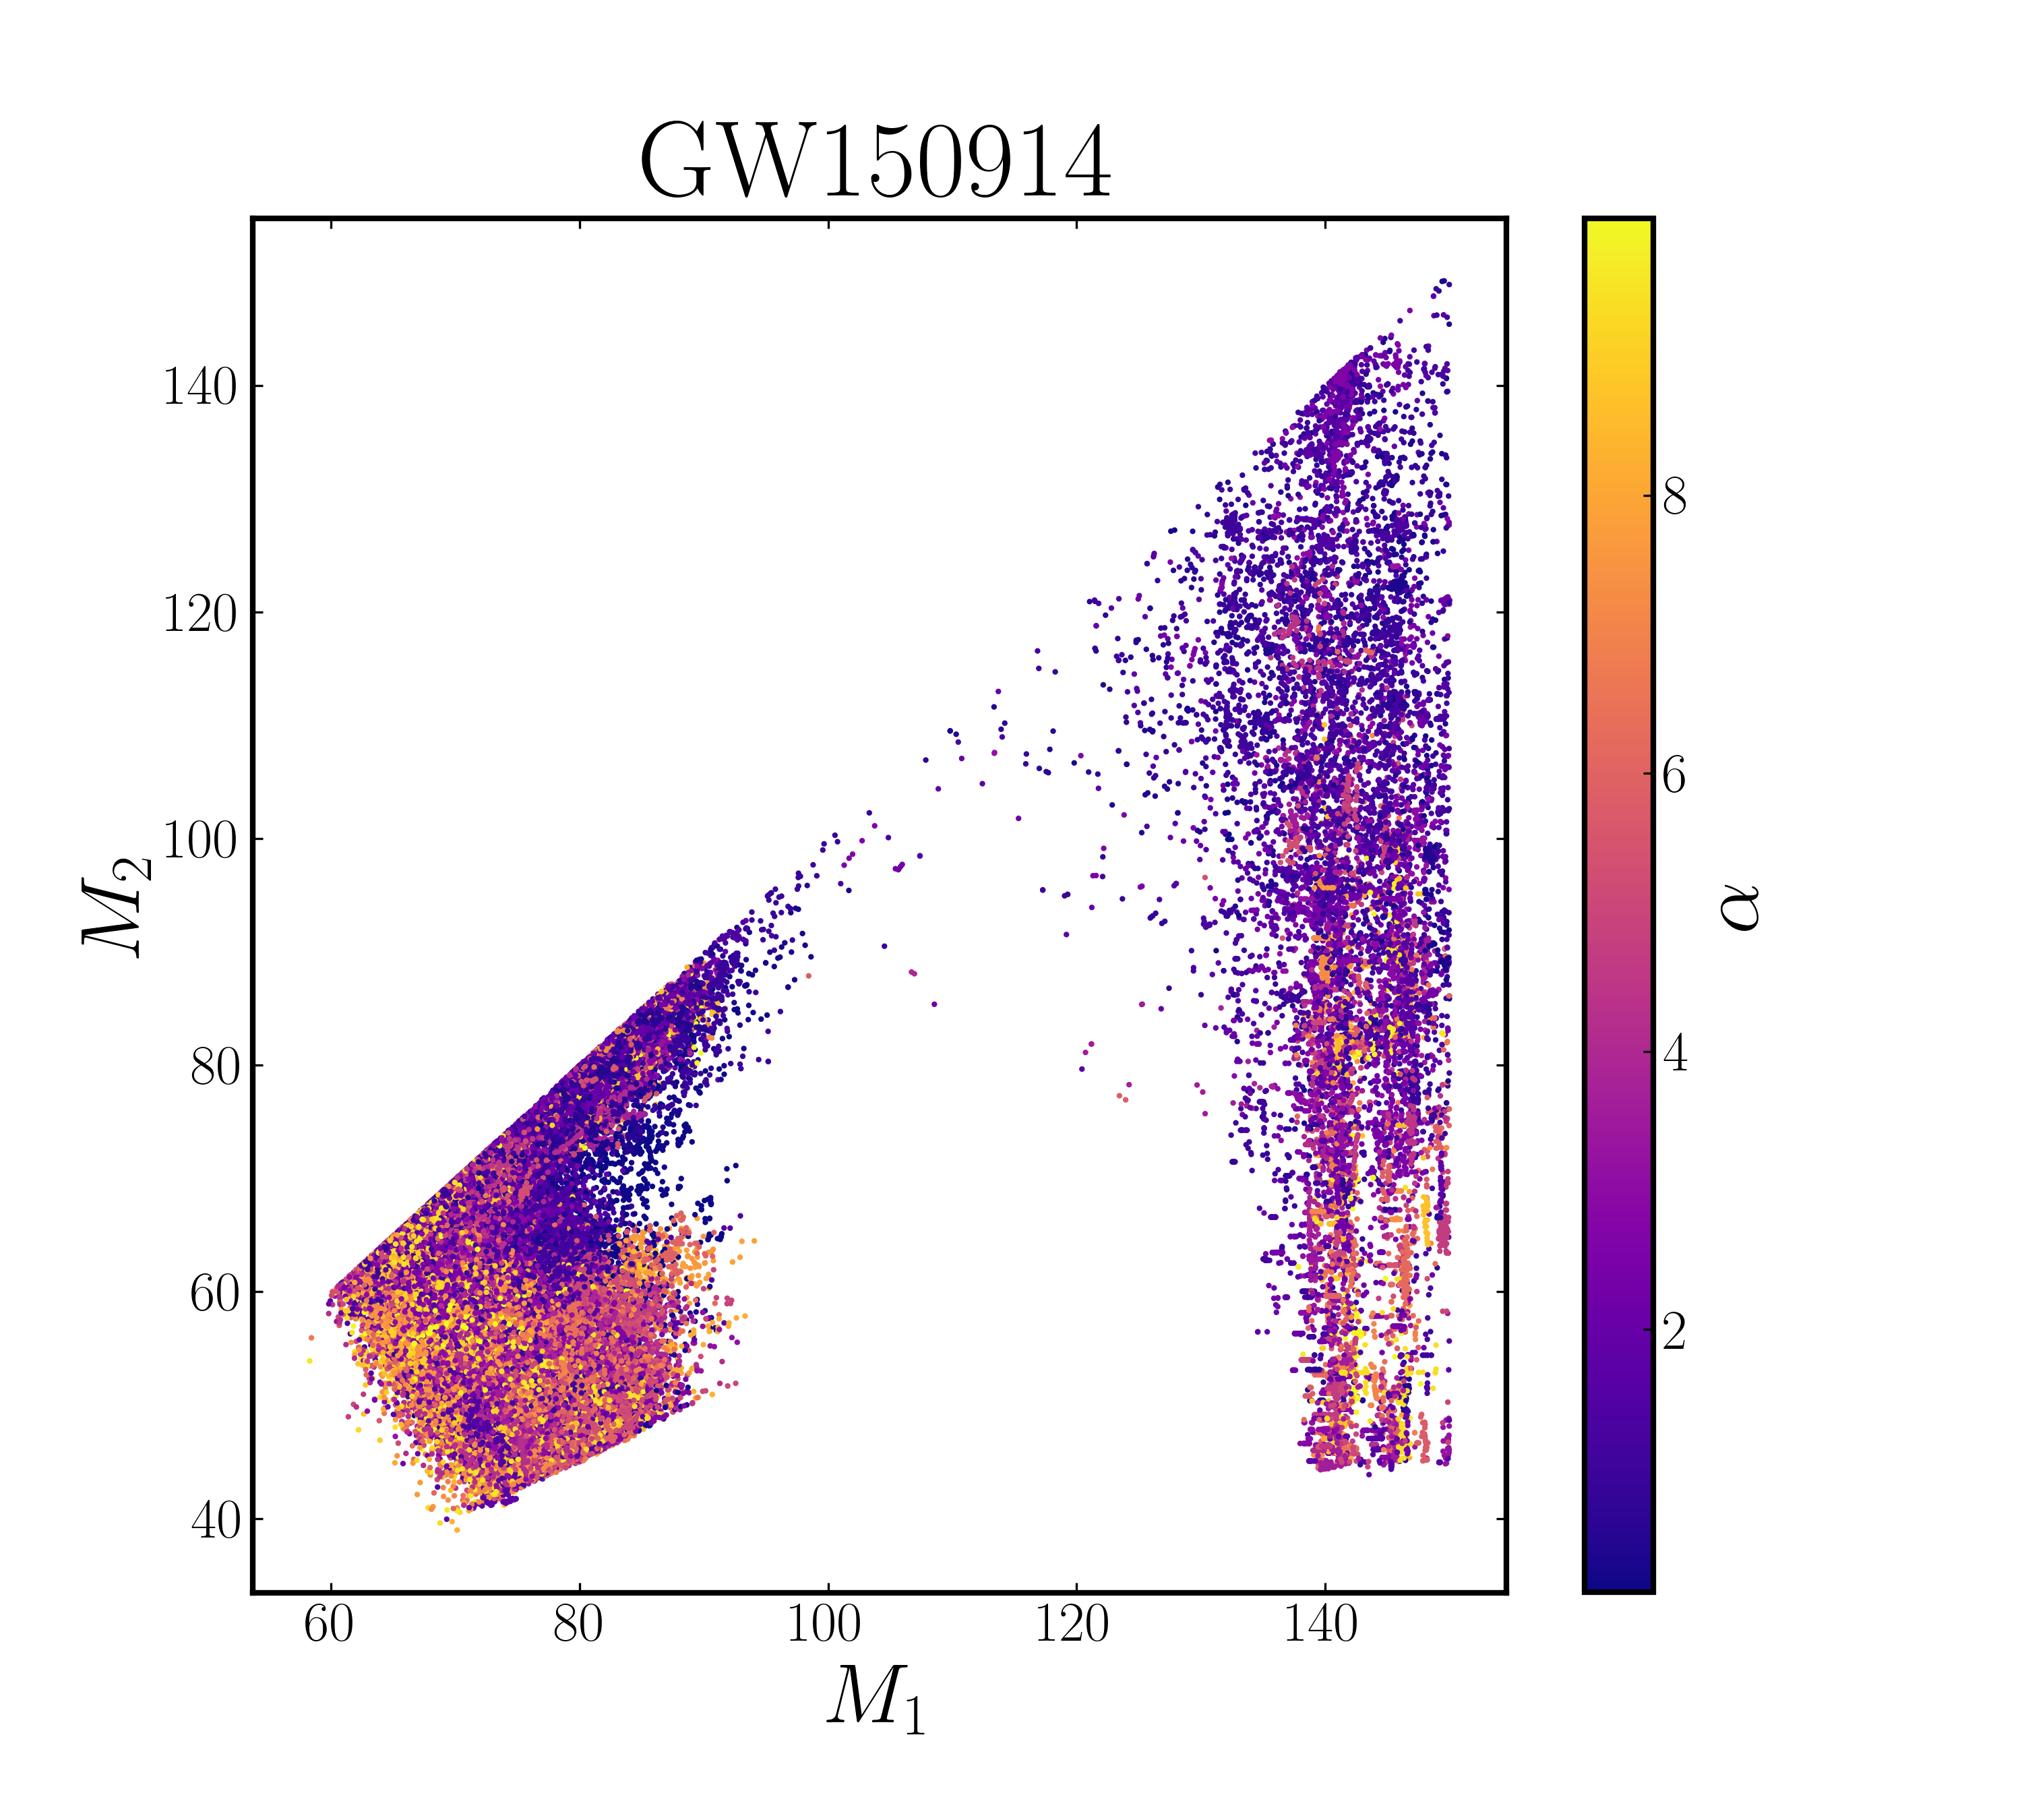
\includegraphics[width=0.49\textwidth]{static/GW150914_m1m2alpha.png}
\caption{The posterior samples of GW150914 in the progenitor masses space, colorcoded by the common envelope efficiency $\alpha$ for that sample.}
\label{fig:GW150914_m1_m2_alpha}
\end{figure}

\begin{figure}
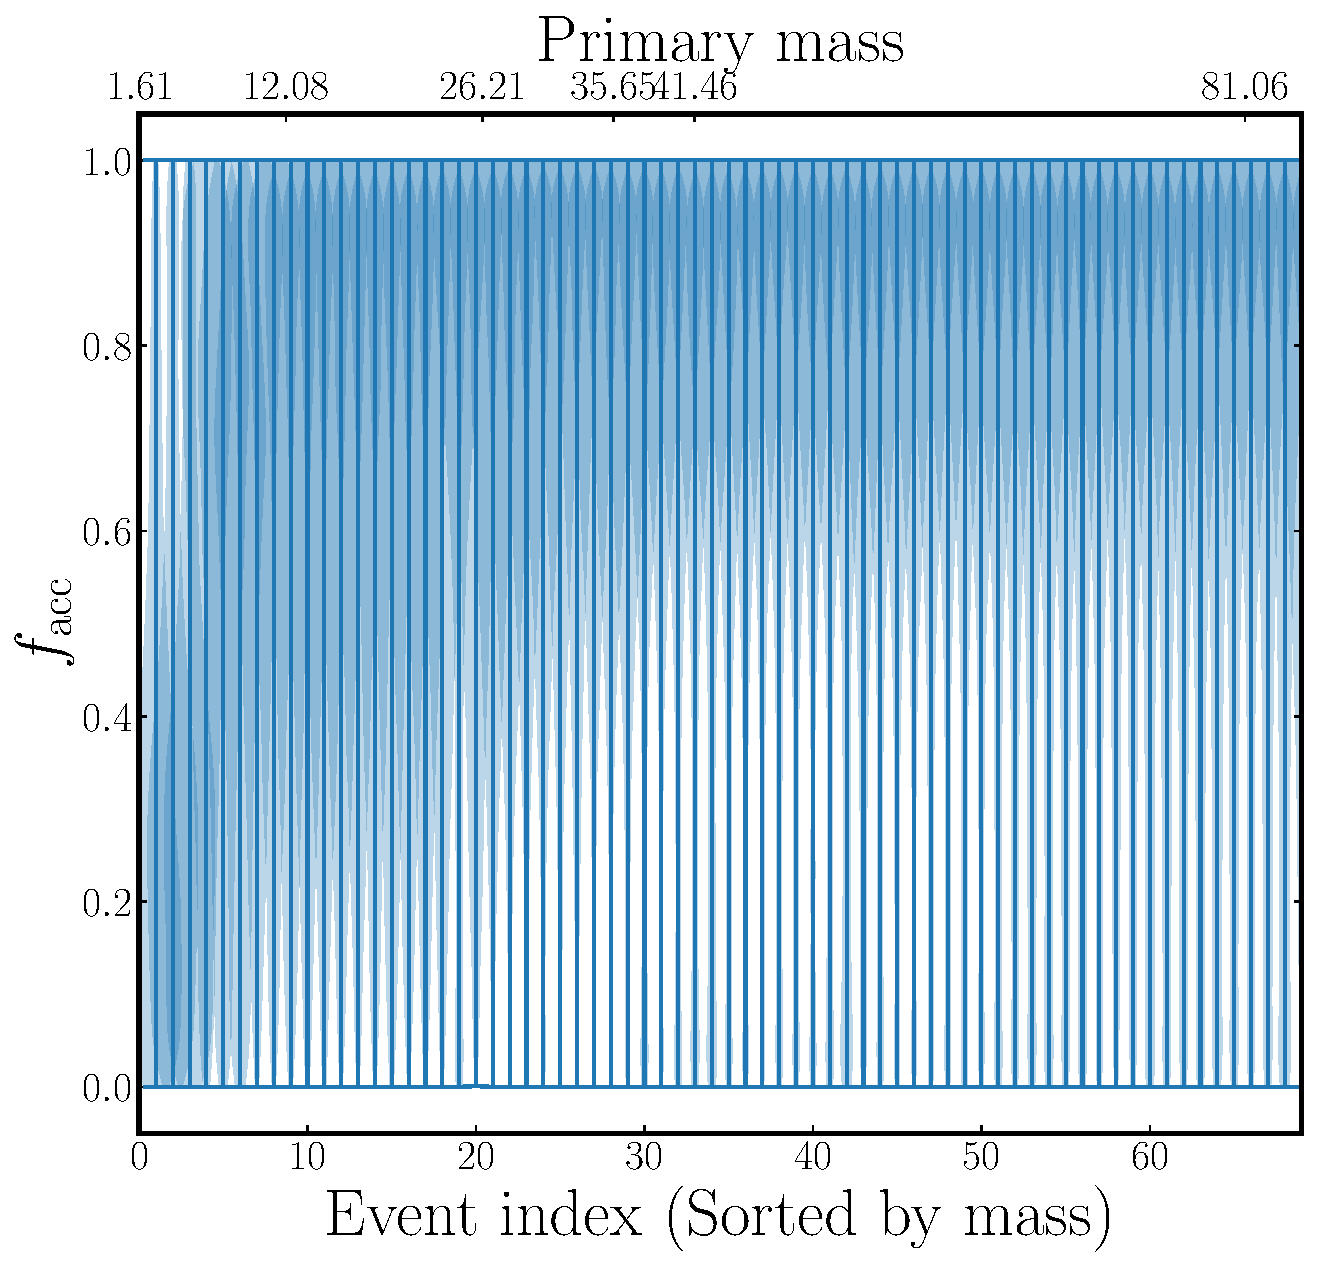
\includegraphics[width=0.49\textwidth]{static/GWTC3_alpha_mass.pdf}
\caption{This figure is ugly as fucked now. Let's change it in later iteration}
\label{fig:GWTC3_alpha_mass}
\end{figure}

\kw{Talk about implication on single event posterior.}
The most important point in this paper is illustrated in figure \ref{fig:GW150914_m1_m2_alpha}.
We can see the posterior samples in $M_1-M_2$ space are spatially correlated with $\alpha$,
this means if we fixed the value of $\alpha$ instead of allowing it to jointly vary with all other parameters,
we would miss the samples that do not match the chosen value of $\alpha$.
By folding in the hyper-parameters into the root-finding algorithm,
we can capture the correlation between 
\kw{Dartboard comparsion} Comparing our result with 

\kw{Discuss implication in population.}
To illustrate the potential benefit of our method in the population, we perform the same analysis for most of the events in GWTC3.

Plotted in figure \ref{fig:GWTC3_alpha_mass} is the constraint of $f_{\rm acc}$ for all the events included in the analysis sorted by the median of their inferred primary mass in the observable space.
Note that some events on the extreme of the mass spectrum did not pass the KL divergence test we proposed in section \ref{sec:method}.
\kw{Double check}On the low mass end, the events are more subjected to random fluctuation because natal kick is less modulated by fallback in lighter system, so the reprojected 
On the high mass end, \texttt{COSMIC} struggles to produce events in the pair instability supernova mass gap,
so the posterior in the evolutionary parameter space only correspond part of the posterior in the observable space, therefore events beyond the PISN mass gap has higher KL divergence.


The point of figure \ref{fig:GWTC3_alpha_mass} is to show this method could reveal the correlation between the primary mass in the BBH and the common envelope efficiency.
A careful treatment of each event in the catalog and discussion related the physical implication of figure \ref{fig:GWTC3_alpha_mass} is beyond the scope of this paper,
therefore we defer a detail study of the physics related to the population of GW events in the future.



\section{Discussion}
\label{sec:discussion}


We present a new pathway to understand binary evolution with GW events in this paper.
Instead of forward modelling an assumed distribution of initial binary to the observed population,
we find the corresponding evolutionary parameters for each GW events. 
In this work we first showcase the power of the proposed method with GW150914.
We show the joint posterior of the two events' progenitor parameters and hyper-parameters.
In particular, to the authors' knowledge, this is the first time the correlation between progenitor parameters and hyper-parameters is explored.
Our work is not only a more efficient way to study GW events' progenitors,
but also allows the possibility of measuring the astrophysics related the binary evolution, especially in capturing the correlation between different hyper-parameters.

To further illustrate the power of the method, we show the inferred common envelope efficiency depends on the progenitor masses.
The most obvious advantage our method provides is it returns the joint posterior distribution of progenitor parameters and hyper-parameters for each event.
This enables a data-driven way to study the distribution of hyper-parameters,
i.e. once we have a catalog of events, each has their own set of posterior in the hyper-parameter space,
we can employ common techniques such as hierarchical Bayesian analysis to fit a population model to the distribution of hyper-parameters,
without making specific assumptions such as fixing the hyper-parameters for all types of event.

% Rate analysis is now just counting, like what's done in phenomenological model, instead of forward modelling.
Another perk of our method is the "rate" calculation is now independent of assumed initial condition such as a particular star formation rate model,
which is a dominant factor of uncertainty for rate prediction in the past.
Once we have pull back the GW event posterior from the observable space to the evolutionary parameter space,
we can apply the same methods we use to account for the rate in the observable space.
In the observable space, the overall rate is basically a normalization that is defined in the local universe i.e. the local merger rate. \kw{cite}
In the evolutionary parameter space, we can instead fit for the production rate of merger events at some redshift.


% Single formation channel and fundamental limitation on that.
While our method allows data-driven exploration of the hyper-parameters space for the first time, there are a number of improvements can be implemented in future studies.
In this study we use only \texttt{COSMIC} as our evolutionary function, which by design cannot explain all the events in GWTC3.
For example, event with either of the component mass larger than the PISN gap such as GW190521 cannot be explained by \texttt{COSMIC}.
Alternative channels such as dynamic formation channel will be needed to explain some subset of the events in GWTC3.
As pointed out in the literature \kw{Cite mike}, it is unlikely that all the observed events in GWTC3 can be explained by a single formation channel.
As GW detectors sensitivity increase, we expect to see more and more events that are unusual in some way.
Therefore, having a self-consistence population synthesis code that contains multiple formation channels is essential to accommodate the growing catalog of GW events.
In this paper, our main focus is to illustrate the concept of "back-propagating" GW events posterior sample in this work,
highlighting the capability of our method and motivating the community to build the next generation population synthesis code that can work with our method.
To avoid cluttering of focus, we discuss the physical implication of the result presented in this work under our specific assumption (i.e. using \texttt{COSMIC} as our evolutionary function) in a companion paper.


% Randomness paragraph
Due to the implicit definition of random variables in \texttt{COSMIC}, our evolutionary function is stochastic.
This introduces significant inefficiency in our root-finding and sampling algorithm.
The main stochasticity in \texttt{COSMIC} comes from natal kick, which significantly affect the evolution pathway of low mass events such as BNS events.
The effect of natal kick is suppressed for heavier mass events due to fallback.
This means events with lighter masses are subject to stochasticity of the function,
where the sampling process for heavier events behaves as if the evolutionary function we use are deterministic.
% Indeed, we see this behavior in a couple of case studies.
% For heavy event such as GW150914, the reprojected posterior agrees with the data posterior.
% For light event such as GW170817, although during the root-finding process the convergence criteria is met,
% the reprojected posterior does not agree with the data posterior.
Due to computational limitation, we only try 1000 different initial guesses per posterior sample in the root-finding process.
This means any posterior sample that has a probability of merging rarer than 1 in 1000 could be missed.
Obviously the problems which comes with the randomness can be alleviated by performing more tries per posterior sample,
but this is not scalable in practice.
On top of limitation in efficiency, some formation channels require explicit control of random variables by construction.
For example, in a dynamical formation scenario such as binaries that form in a globular cluster,
each binary has some probability of undergoing a multi-body encounter with another member in the cluster.
These encounter probability distributions are either studied with direct N-body simulations or semi-analytical methods.
In both cases, each member of the cluster is no longer completely independent of the other members, but coupled through the encounter probability distribution.
By studying the encounter probability distribution, we can infer the properties of the environment which the binary lives in.
This can only be done if we have explicit control over the random variables that characterize the encounter probability distribution.

% Need for selection bias to recover intrinsic distribution



% Gradient decending in the evolutionary parameter space is much more efficent than rejection sampling.
% Potential pitfall of interpreting this result.
% Need for full autodiff.

% By leveraging gradient-based optimization strategy, obtaining posterior samples in the evolutionary parameter space is much more efficient than rejection sampling.
% In each optimization step during the root-finding process, the current state of the guess and its gradient provide useful information about where the root might be.
% In contrast to sampling algorithm, which discard the sample whenever it is not accepted.
% This greatly benefit the efficiency of the root-finding process.
% On the other hand, this method is not a sampling algorithm, but a coordinate transform of the posterior samples.
% One should pay extra caution in interpreting the posterior samples in the evolutionary parameter space.
% Since posterior samples in the observable space can in principle have multiple roots in the evolutionary parameter space,
% the relatively weighting of these roots becomes ambiguous when the number of roots is large.
% For example, should we consider roots that are close to each other a single root or multiple roots?
% If we have two clusters of roots, the relative number of roots within each cluster would determine the relative weight of each mode.
% Note that since they both map to the same observable posterior sample within the acceptance threshold, all weighting assigned are equally valid from a "matching data" standpoint.
% This leave the interpretation of the posterior in the evolutionary parameter space ambiguous.
% In our case, we found empirically each posterior sample may at most only correspond to a handful of roots (most of the posterior samples have a unique root.), therefore we choose to assign equal weight to each root.

% The potential reason for the good agreement between MCMC and the root finding is due to the behavior of posterior in the evolutionary parameter space are larger determined by the posterior distribution in the observable space instead of multiple possible roots per posterior sample.
% We have also compared two MCMC results, one is initialized using the roots and another is initialized using samples drawn from a uniform prior.
% We found empirically the MCMC result using the roots as initialization converges at least an order of magnitude faster than the uniform prior initialization.
% This makes sense since the roots basically eliminate the long burn-in needed to go from random location in the evolutionary parameters to the most probable region.
% We leave a detail comparison between this method and direct sampling to future studies.

Another technical note is we use finite differencing to estimate the gradient of the objective function, which could be a significant source of error near transition points in the evolutionary parameter space.
Also, finite differencing is increasing inefficiency as we increase the dimensionality of the problem.
To improve the accuracy and efficiency in estimating the gradient of objective function, automatic differentiation is a promising feature that modeler should consider incorporating in their population synthesis code in the future.


To summarize, we propose a novel method to recover the posterior samples in the evolutionary parameter space for each GW event.
We point out hyper-parameters in the usual population synthesis simulation context are not actually parameters related to the population,
but parameters about the evolutionary function.
This means the binary evolution functions can be constrained on an individual event basis.
We "back propagate" the posterior in the observable space to the evolutionary parameter space,
thus allowing us to study hyper-parameters and its correlation with progenitor parameters in a data-driven manner.
Our method makes less assumption than the traditional forward modelling approach,
which often fix the hyper-parameters across the entire population.
Since we are not limited to the fix hyper-parameters assumption, we can explore the behavior of the hyper-parameters across the population much more efficiently.
While our work lay down a data analysis pathway to understand the population of GW events,
no physics can be learned without a comprehensive physical model.
We hope this letter would motivate the community to build the next generation population synthesis codes that have the following properties:
first, they should have explicit control over the random variables so marginalizing over random variables can be done more precisely;
second, they should be as automatically differentiable as much as possible so exploring the evolutionary parameter space is efficient.
Combining this work and the next generation population synthesis code,
we can explore the full parameter space of binary evolution models with the next-generation GW detectors network in the near future.


\section{Acknowledgement}

\bibliography{bib}

\end{document}
